\subsection{Electromagnetic wave and Poynting vector}

\begin{frame}{Electromagnetic wave and Poynting vector}
    \begin{columns}
    \column{0.5\textwidth}
    \vspace{-4mm}
    \begin{itemize}
        \item Wave equation: 
        \begin{equation*}
            \varepsilon \mu \frac{\partial^2 \mathbf{A}}{\partial t^2} - \nabla^2 \mathbf{A} = 0.
        \end{equation*}

        \item Phase velocity: 
        \( c = (\varepsilon \mu)^{-1/2} = c_0/n \).
        \item Poynting vector: 
        \( \mathbf{S} = \mathbf{E} \times \mathbf{H} \).
    \end{itemize}

    \begin{figure}
        \centering
        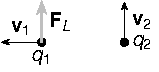
\includegraphics[width=0.5\textwidth]{Figures/Newton_3rd_law.pdf}
        \caption{Newton's 3rd law is wrong with Lorent force because of Poynting vector.}
        \label{fig:Newton_3rd_law}
    \end{figure}
    
    \column{0.5\textwidth}
    \vspace{-6mm}
    \begin{figure}
        \centering
        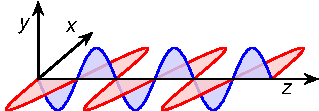
\includegraphics[width=\textwidth]{Figures/Electromagnetic_wave.pdf}
        \caption{Electromagnetic wave.}
        \label{fig:Electromagnetic_wave}
    \end{figure}
    \vspace{-2mm}
    \begin{figure}
        \centering
        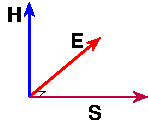
\includegraphics[width=0.5\textwidth]{Figures/Poynting_vector.pdf}
        \caption{Poynting vector.}
        \label{fig:Poynting_vector}
    \end{figure}


    \end{columns}
\end{frame}